\documentclass[12pt]{article}
\usepackage[ngerman]{babel}
\usepackage[utf8]{inputenc}
\usepackage[round,authoryear]{natbib}
\usepackage[hyphens]{url}
\usepackage{amssymb}
\usepackage{hyperref}
\usepackage{float}
\usepackage[]{graphicx}
\usepackage[all]{hypcap}
\usepackage{titlepic}
\usepackage{caption}
\usepackage{subcaption}
\usepackage{titling}
%\pagenumbering{gobble}
\title{AVPRG Konzept \glqq Abakus\grqq}
\setlength{\droptitle}{-2em}
\author{Stefan Schäfers (2175460), Julian Roosch (2203745)}
\begin{document}
\maketitle
\begin{abstract}
Ein Abakus ist ein mechanisches Rechenhilfsmittel, welches Kugeln, oft aus Holz oder Glas, verwendet, die auf einer horizontalen Strecke verschoben werden können. Je nach Ausführung wird auch die Bezeichnung Zählrahmen verwendet.

In unserem Projekt soll ein Abakus zur Steuerung von Parametern in Audiosoftware verwendet werden.

\end{abstract}
\section{Beschreibung aus Nutzersicht}
%nutzer verschiebt kugeln auf abakus
%verschiebt werte auf virtuellem interface -> tangable schieberegler
%Ein Nutzer soll an einem Abakus ähnelndem Objekt farbige Kugeln auf vertikal übereinander angeordneten Stangen frei bewegen können. Je eine Kugel beschreibt in Relation zu ihrer Position auf der jeweiligen Stange einen Wert. Dieser Wert soll anschließend an eine Schnittstelle weitergeleitet werden, damit mit den Kugeln ein Interface gesteuert werden kann. Jede Kugel stellt somit eine Art \glqq tangable Schieberegler\grqq dar.
Ein Nutzer kann an einer Art Abakus kleine farbige Kugeln auf vertikal übereinander angeordneten Stangen verschieben. Jede Reihe stellt dabei einen eigenen Parameter dar, jede Kugel mit ihrer Stange fungiert als eine Art “tangable Schieberegler”. In Relation zu der Position repräsentieren die Kugeln auf ihrer jeweiligen Stange einen Wert, der anschließend an eine Schnittstelle weitergeleitet werden soll, um damit ein Interface zu steuern. \begin{figure}[H]
\begin{center}
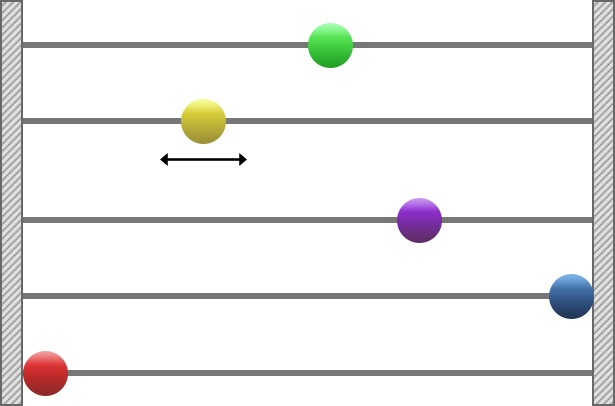
\includegraphics[width=0.6\linewidth]{AbakusSK_Farbe.png}
\caption{Veranschaulichung der Bedienung}
\end{center}
\end{figure}Durch das Verschieben der Kugeln werden also die Werte des Interfaces verändert und mittels Midi weitergesendet - so entsteht aus dem Abakus ein kleiner Midi-Controller. Die gesendeten Midi-Werte kann der Nutzer beispielsweise dazu verwenden, den kleinen Synthesizer aus AVPRG zu steuern oder er kann die Midi-Werte mit beliebigen Parametern in einer DAW verknüpfen.



\section{Technisches Konzept}
%farbige kugeln übereinander angeordnet
%gut beleuchtet, weißer hintergrund
%Jede auf dem Abakus befindliche farbige Kugel wird von einer Kamera erfasst, die sich unmittelbar vor dem Abakus positioniert wird. Die Einzelbilder werden in einem Analyseprogramm mit Hilfe der Programmbibliothek \glqq OpenCV\grqq ausgewertet. Hier findet die Objekterkennung der Kugeln anhand ihrer Farbe statt. Wichtig für die Farben der Kugeln ist, dass die Farben zweier vertikal benachbarten Kugeln möglichst unterschiedlich sind. Unterschiedliche Farben bedeutet hier, dass (?). Mit dem horizontalen Bewegen einer Kugel von links nach rechts soll ein Wert von 0\% bis 100\% eingestellt werden können. Dieser Wert wird aus der ermittelten Position der Kugel generiert und wird anschließend entweder über einen korrespondierenden MIDI-Wert an eine DAW geschickt oder direkt an die variablen Einstellungsmöglichkeiten des Synthesizers aus der AVPRG Vorlesung weitergeleitet.
%Erfassung der Kugeln durch Kamera
%Positionsermittlung mit hilfe von OpenCV
%Fehlervermeidung => Verkleideter Hintergrund, Vermeidung bestimmter Farben
%Filterung, Auswertung der Positionen => Skalierung/Auswertung => Weiterleitung

Jede auf dem Abakus befindliche farbige Kugel wird von einer Kamera erfasst, die sich unmittelbar vor dem Abakus positioniert wird. Der Abakus wird dabei gut beleuchtet, damit die Kamera möglichst kontrastreiche Bilddaten erhält. Um weitere Fehlerquellen zu vermeiden wird der von der Kamera erfasste Bereich einfarbig Verklediet (Karton, Papier, Pappe o.ä.), damit die Farberkennung außerhalb des gewünschten Bereiches reduziert wird (Erkennung der Farbe(n) der Kugeln in der Umgebung vermeiden).
\begin{figure}[H]
\begin{center}
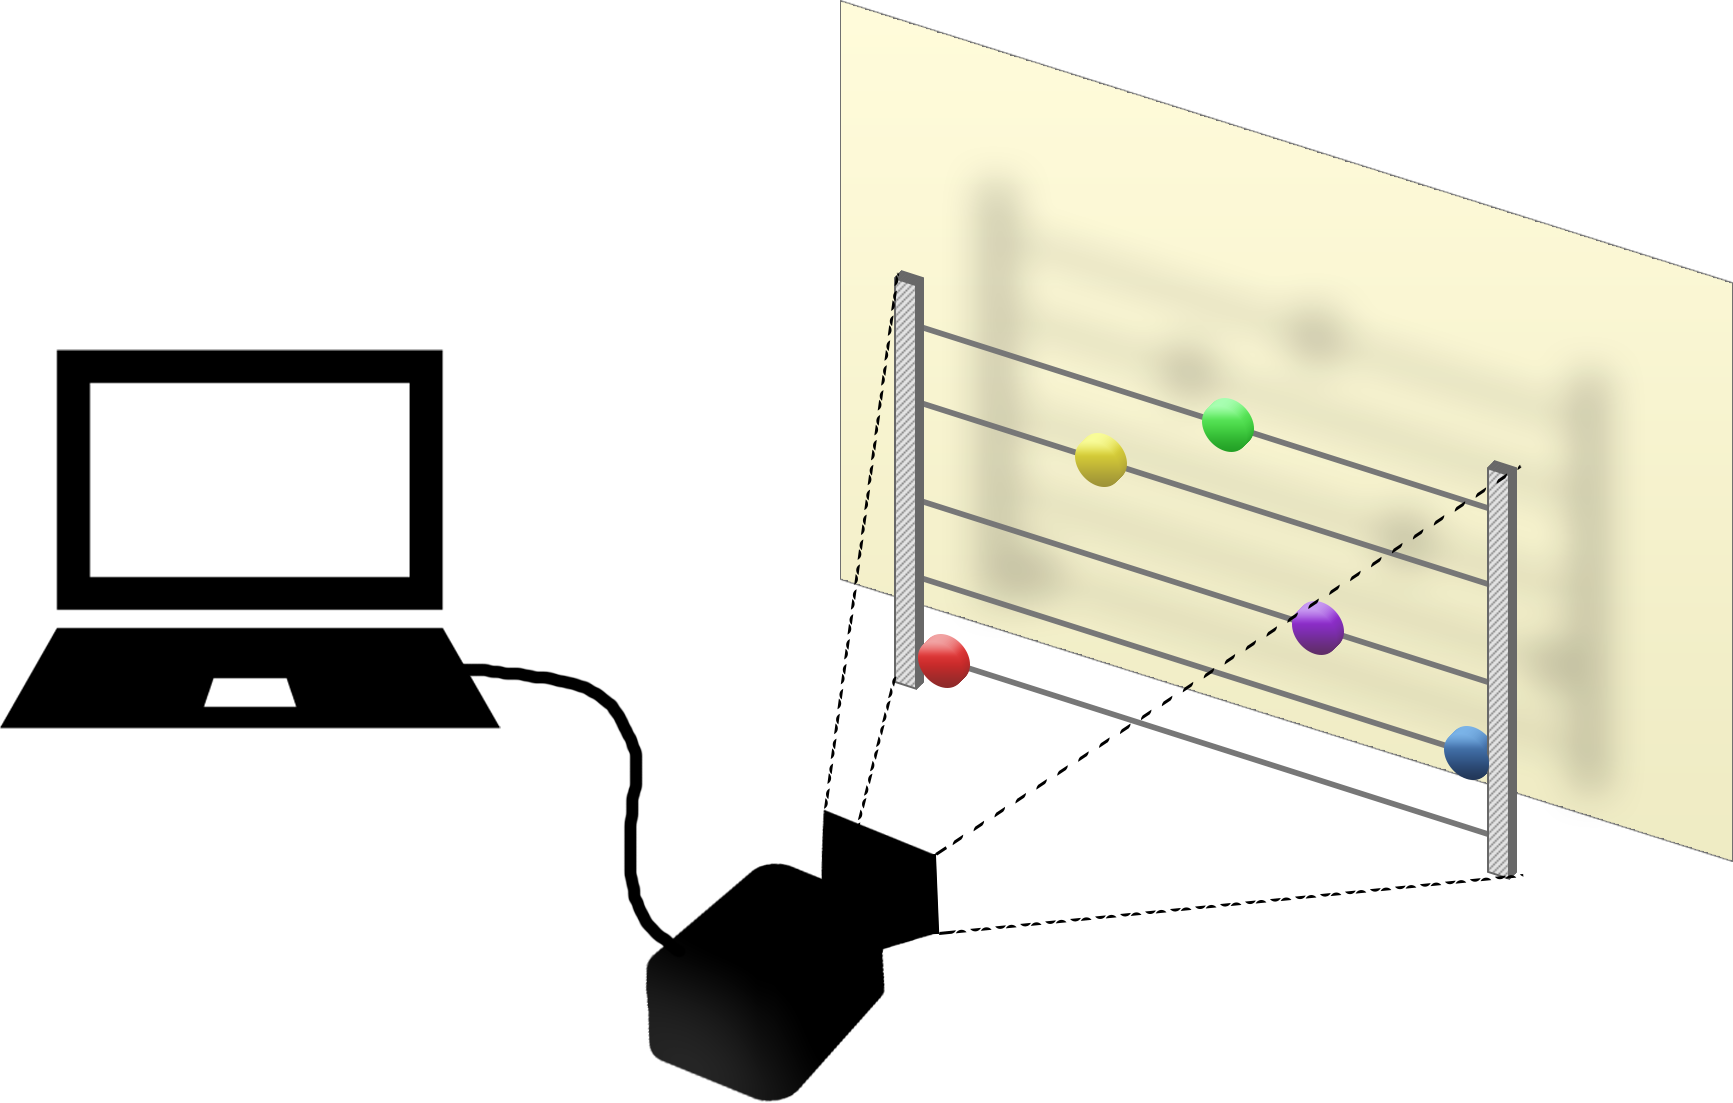
\includegraphics[width=0.6\linewidth]{Ges_Perspektive.png}
\caption{Schematische Darstellung des Aufbaus}
\end{center}
\end{figure}
Damit es bei der Bedienung durch einen Nutzer nicht zu Fehlern kommt, werden hautfarben ähnliche Farben (rot, orange, gelb) bei den Kugeln ausgeschlossen. Die von der Kamera aufgezeichneten Einzelbilder werden in einem Analyseprogramm mit Hilfe der Programmbibliothek \glqq OpenCV\grqq ausgewertet. Wenn die Filterung und somit die Erfassung der Positionen der Kugeln abgeschlossen ist, werden die Positionen ausgewertet. Wie oben bereits erwähnt, definiert eine Kugel den Wert des Reglers über die Entfernung zur linken bzw. rechten Seite. Jede Reihe beschreibt dabei den Wert einer bestimmten Variable. Abhängig von der Variable, die mit dem Regler angesteuert werden soll, wird der von der Kugel dargestellte Wert auf einen bestimmten Wertebereich abgeblidet und/oder skaliert. Diese Daten werden direkt an eine Audiosoftware weitergeleitet, um die Bedienung des Abakus hörbar zu machen.
 \begin{figure}[H]
\begin{center}
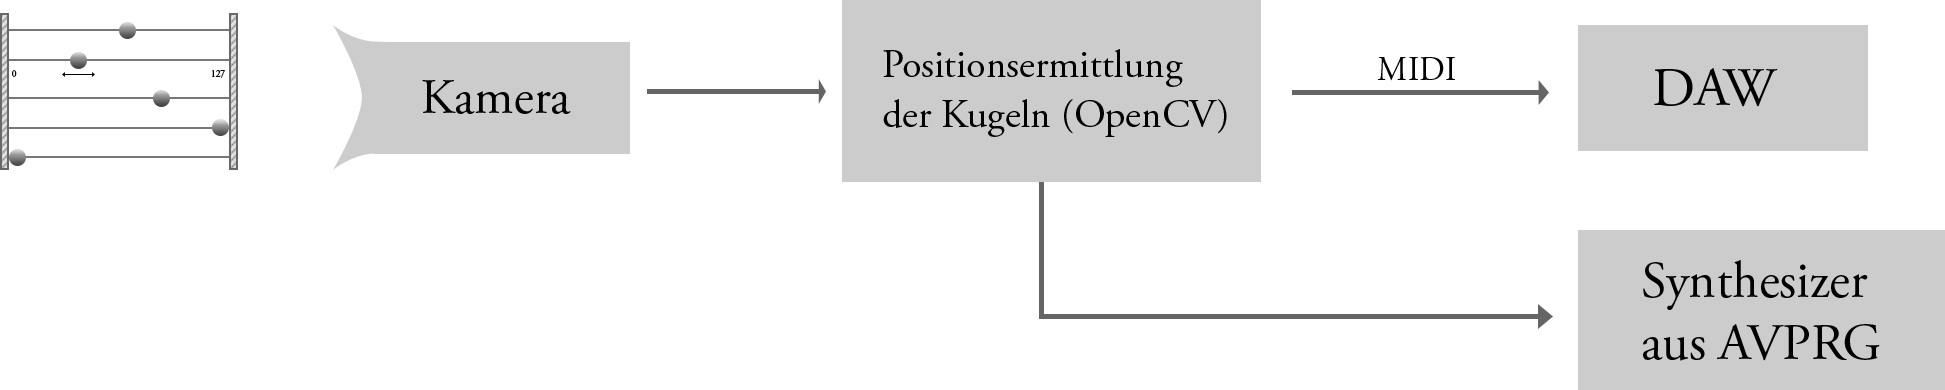
\includegraphics[width=0.8\linewidth]{Gruppe_6.png}
\caption{Verlauf der Aufnahme der Daten bis zur Auswertung}
\end{center}
\end{figure}


%Die Einzelbilder werden in einem Analyseprogramm mit Hilfer der Programmbibliothek \glqq OpenCV\grqq ausgewertet. Hier findet die Objekterkennung der Kugeln anhand ihrer Farbe statt. Um die Farberkennung und die Filterung und somit das Tracking der Kugeln zu vereinfachen, wird der Hintergrund einfarbig verkleidet (weiß/grau) und die Szene gut ausgeleuchtet. Damit es bei der Bedienung durch einen Nutzer nicht zu Fehlern kommt, werden hautfarben ähnliche Farben (rot, orange, gelb) bei den Kugeln ausgeschlossen. 
%Wenn die Filterung und somit die Erfassung der Positionen der Kugeln abgeschlossen ist, werden die Positionen ausgewertet. Wie oben bereits erwähnt, definiert eine Kugel den Wert des Reglers über die Entfernung zur linken bzw. rechten Seite. Dieser (prozentuale) Wert kann nun auf einen Wertebereich abgebildet und/oder, in Abhängig von der Funktionalität, skaliert werden. Diese Daten werden direkt an eine Audiosoftware weitergeleitet, um die Bedienung des Abakus hörbar zu machen.



\end{document}